%% ENCODING UTF-8
\documentclass[a4paper,11pt]{article}

%%%%%%%%%%%%%%%%%%%%%%%%%%%%%%%%%%%%%%%
%%%%%%%%%%%%%%%%%%%%%%%%%%%%%%%%%%%%%%%
%
% Latex Template for Marie Curie CIG
%
% NOTE this is not an official template; adjust margins, formatting
% etc as required
%
%%%%%%%%%%%%%%%%%%%%%%%%%%%%%%%%%%%%%%%
%%%%%%%%%%%%%%%%%%%%%%%%%%%%%%%%%%%%%%%

%% Arial-like fonts
%\renewcommand{\rmdefault}{phv} 
%\renewcommand{\sfdefault}{phv} 

\usepackage[T1]{fontenc}
\usepackage[utf8]{inputenc}
\usepackage[margin=2.5cm]{geometry}
\usepackage[usenames,dvipsnames]{color}
\usepackage{tabularx}
\usepackage{graphicx}
\usepackage{xspace}
\usepackage{eurosym}
\usepackage{fancyhdr}
\pagestyle{fancy}
\usepackage{datetime}
\usepackage{lastpage}
\usepackage{pdfpages}
\usepackage[numbers,sort&compress]{natbib}
\usepackage[colorlinks=true, linkcolor=BrickRed, citecolor=Blue, urlcolor=Blue, filecolor=Blue]{hyperref}
\input{jdefs.tex}

\renewcommand{\thesection}{B\arabic{section}} 

\newcommand{\content}[1]{\emph{#1}\\} 

\bibliographystyle{JHEP_pat}
\bibpunct{[}{]}{,}{n}{ }{,}

\newif\ifMyDraft% boolean variable whether or not to show xcomments
\MyDraftfalse%    default should be false

%%%%%%%%%%%%%%%%%%%%%%%%%%%%%%%%%%%%%%%
%%%%%%%%%%%%%%%%%%%%%%%%%%%%%%%%%%%%%%%
%%%% ADJUST HERE

\newcommand{\projectname}[0]{GAMBIT Startup\xspace} 

\newcommand{\mytitle}{Astroparticle Searches and Treasure Maps for Particle Physics Beyond the Standard Model}
% set MyDraft to true in order to get comments for the sections displayed, the build date, etc...
%\MyDrafttrue
%%%% END OF ADJUST HERE
%%%%%%%%%%%%%%%%%%%%%%%%%%%%%%%%%%%%%%%
%%%%%%%%%%%%%%%%%%%%%%%%%%%%%%%%%%%%%%%

%%%%%%%%%%%%%
\ifMyDraft % iftrue: this is a draft
  
\newenvironment{xcomment}{\em}{}
  \lhead{}
  \chead{\projectname{} -- version of \today{}, \currenttime}
  \rhead{}
\else
  \usepackage{xcomment}
  \lhead{}
  \chead{\projectname}
  \rhead{}
\fi

\title{\mytitle}
%%%%%%%%%%%%%

%%%%%%%%%%%%% the cover STARTPAGE and ENDPAGE macro

\newcommand{\cover}[1]{%

\newpage
\begin{center}
\LARGE
\vspace{6cm}

\textbf{#1}
\vspace{2cm}

PEOPLE

MARIE CURIE ACTIONS
\vspace{2cm}

\textbf{Marie Curie Career Integration Grants (CIG)}

\textbf{Call: FP7-PEOPLE-2013-CIG}

\vspace{4cm}

PART B
\vspace{2cm}

\mytitle
\vspace{1cm}

``\projectname''

\cfoot{}

\end{center}

\newpage
} 
%%%%%%%%%%%%% end of cover STARTPAGE and ENDPAGE macro

%%%%%%%%%%%%%%%%%%%%%%%%%%%%%%%%%%%%%%%%%%%%%%%%%%%%%%%%%%%%%%%%%%%%%%%%%%%%%%%%%%%%%%%%
%%%%%%%%%%%%%%%%%%%%%%%%%%%%%%%%%%%%%%%%%%%%%%%%%%%%%%%%%%%%%%%%%%%%%%%%%%%%%%%%%%%%%%%%
%%%%%%%%%%%%%%%%%%%%%%%%%%%%%%%%%%%%%%%%%%%%%%%%%%%%%%%%%%%%%%%%%%%%%%%%%%%%%%%%%%%%%%%%
\begin{document}

\cover{STARTPAGE}
%%%%%%%%%%%%%%%%%%%%%%%%%%%%%%%%%%%%%%%%%%%%%%%%%%%%%%%%%%%%%%%%%%%%%%%%%%%%%%%%%%%%%%%%
\pagenumbering{roman}
\cfoot{Part B -- Page \thepage}
\tableofcontents

\newpage
%%%%%%%%%%%%%%%%%%%%%%%%%%%%%%%%%%%%%%%%%%%%%%%%%%%%%%%%%%%%%%%%%%%%%%%%%%%%%%%%%%%%%%%%

\pagenumbering{arabic}
\cfoot{Part B -- Page \thepage\ of \pageref{LastPage}}

\begin{xcomment} 
Warning: the comments are turned on. All directives and guidelines appear.

To turn them off, comment the line:\\ 
\verb|\MyDrafttrue|\\

\end{xcomment} 


%%%%%%%%%%%%%%%%%%%%%%%%%%%%%%%%%%%%%%%%%%%%%%%%%%%%%%%%%%%%%%%%%%%%%%%%%%%%%%%%%%%%%%%%
%%%%%%%%%%%%%%%%%%%%%%%%%%%%%%%%%%%%%%%%%%%%%%%%%%%%%%%%%%%%%%%%%%%%%%%%%%%%%%%%%%%%%%%%
\section{Scientific and Technological Quality}

\begin{xcomment}  
Maximum 7 pages
\end{xcomment}

%%%%%%%%%%%%%%%%%%%%%%%%%%%%%%%%%%%%%%%%%%%%%%%%%%%%%%%%%%%%%%%%%%%%%%%%%%%%%%%%%%%%%%%%
\subsection{Research and technological quality, including any interdisciplinary and multidisciplinary aspects of the proposal}
\label{outline}

\begin{xcomment}  
Start out by defining the research area of the intended research
objectives. This description should give an overall picture of all
research activities that will be performed (including possible
developments or alternatives) within the work agreement that is the
condition for the CIG grant, irrespective of the source of funding.

Outline the research objectives against the background of the state of
the art, and the results hoped for. Give a clear description of the
state-of-the-art of the research topic. Describe the scientific,
technological or socio-economic reasons for carrying out further
research in the field covered by the project. If relevant, provide
information on interdisciplinary / multidisciplinary and/or
intersectorial aspects of the proposal.
\end{xcomment}

The identity of dark matter (DM) and the nature of physics at the TeV energy scale are two of the most pressing and fundamental questions in modern physics.  DM constitutes 80\% of the matter in the Universe and was discovered 80 years ago, but its composition remains a mystery.  With the impending activation of the 14\,TeV Large Hadron Collider (LHC), discovery of the Higgs boson and construction of high-energy astrophysics experiments like the \textit{Fermi}-LAT, HESS-II, IceCube and SuperCDMS, we now stand on the doorstep of the TeV scale.  

Excitingly, many popular DM candidates are intrinsically linked to the appearance at the TeV scale of new physics beyond the Standard Model (BSM) \cite{Jungman96,Bergstrom00,Bertone05}.  A Higgs mass of 125\,GeV itself even compels us to move beyond the Standard Model: theoretically, this value should be orders of magnitude higher if the impact of Standard Model virtual particles is taken into account \cite{Martin,BaerTata}.  If no other particles exist, then the very vacuum of our Universe is also unstable \cite{Degrassi12}, and might undergo a catastrophic energy transition at any moment.  We also know that the Standard Model is incomplete because it does not explain the excess of matter over antimatter in our Universe, nor the fact that neutrinos have mass.

Many different probes are sensitive to BSM physics: direct and indirect searches for DM, accelerator searches, and neutrino experiments.  Experiments such as CRESST \cite{CRESST11}, \textit{Fermi}-LAT \cite{Hooper11,Bringmann12,Weniger130GeV} and PAMELA \cite{Pamelapositron} may even already show tantalising hints of DM.  To make robust conclusions about the overall level of support for different BSM scenarios from such varied sources, a simultaneous statistical fit of all the data, fully taking into account all relevant uncertainties, assumptions and correlations is an absolute necessity.  This `global fit' approach is the one I intend to follow in my appointment at Imperial College London.  Such holistic analyses exploit the synergy between different experimental approaches to its maximum potential, squeezing every last statistical drop of information possible from each experiment.  Robust analysis of correlated signals, in a range of complementary experiments, is \textit{essential} for claiming a credible discovery of DM or new physics at the TeV scale -- and indeed, even for definitively excluding theories.  This `win-win' situation is a particular feature of a global fit analysis, as even non-detections provide crucial physical insight into which theories and parameter regions are disfavoured.

This is an extremely demanding and interdisciplinary task, existing on the cusp of theory and experiment, astronomy and particle theory -- and requiring excellent understanding not only of the theories and experiments involved, but also many specialised statistical techniques and computer codes.  Astroparticle experimental collaborations have so far carried out such global analyses only with my assistance: the examples to date have been my collaborations with the \textit{Fermi}-LAT \cite{Scott09c}, HESS \cite{Ripken11} and IceCube \cite{IC22Methods} collaborations.  

My intention is to drastically scale up this research program.  Existing global fits \cite{Baltz04, Sfitter, Fittino, Ruiz06, Allanach06, Trotta08, Scott09c, Buchmueller09, Akrami09, AbdusSalam09a, AbdusSalam09b, Ripken11, Allanach11a, Allanach11b, Mastercode11, MastercodeXENON100, MastercodeHiggs, SuperbayesXENON100, Arina11, Pato11, BertoneLHCDD, Fittino12, Mastercode12, Mastercode12b, Roszkowski12, Strege13} cover only a very small subset of interesting models; most have dealt with only the very simplest versions of supersymmetry (SUSY).  This is partly for computational reasons, as efficiently exploring the parameter spaces of more complicated models is extremely time-consuming.  Existing fits have also rarely been truly `global', in that the full range of possible observables and datasets are not included in a detailed way (e.g. indirect searches direct dark matter).  My intention is to massively expand the range of theories to which global fits have been applied, the number of experimental results included in them, and the sophistication of the computational and statistical techniques and tools used to perform them.

This program requires both a leader with experience in all the relevant disciplines, and a team of highly skilled experimental and theoretical specialists to provide expertise and support in specific areas.  In particular, such a team must include members of the actual experimental collaborations themselves, in order to provide state-of-the-art knowledge about specific experimental analyses and datasets.  To this end, I recently founded the Global And Modular BSM Inference Tool (GAMBIT) Collaboration, with 21 other theorists and experimentalists.  GAMBIT will transform the budding field of global fits, by providing a framework in which new theories, observables, likelihoods and scanning algorithms can be quickly, easily and consistently combined in order to completely and rigorously test essentially \textit{any} proposed extension of particle physics beyond the Standard Model.  I am uniquely placed to lead this endeavour, with the extensive cross-disciplinary background in astrophysics and particle physics, theory and experiment, DM phenomenology, statistical and numerical methods required to make this ambitious plan a reality.  

\subsubsection{Scientific Research Objectives}
\label{objectives}

\begin{enumerate}
\setlength{\itemsep}{2pt}
{\it \item Identify the correct theory behind dark matter and TeV-scale BSM physics}
{\it \item Exclude large classes of other viable and popular dark matter and TeV-scale BSM theories}
{\it \item Distinguish between areas of parameter space giving rise to distinct astroparticle phenomena within single BSM theories}
\end{enumerate}

At the present time, the state of knowledge about dark matter and TeV-scale particle physics is essentially just that there is probably some sort of new physics around the TeV scale, that this is not the simplest version of supersymmetry, and that dark matter exists and interacts very weakly with normal matter.  My first two objectives aim to improve on this by either determining precisely what dark matter and the new physics at the TeV scale actually are, and/or ruling out a number of candidate theories that are presently considered viable.  Global fits provide the most complete possible means by which to use all experimental data in the search for dark matter and new physics, and thereby either identify or constrain different particle theories.  

When constraining different theories, one compares the performance of global fits in different parts of the same parameter space.  This indicates which parameter areas are favoured, and to what extent.  This also indicates which physical processes dominate various observables within that theory (e.g. if the DM relic density is set by DM-DM annihilation or DM co-annihilation with another particle).  This is the third goal above.

My research program will provide global fits of unprecedented accuracy, completeness and breadth, allowing me to address these three objectives far better than has been done before.

\subsubsection{Community Research Objectives}
\label{community}

There are three main ways I intend to make this research program impact the scientific community, beyond the direct scientific results it will reproduce.

\begin{enumerate}
\setlength{\itemsep}{2pt}
\setcounter{enumi}{3}

{\it \item Create and distribute a public suite of software tools that allows new theories, observables and datasets to be easily analysed in a global statistical fit}

A very timely component of this project is the development and public release of the GAMBIT software.  The GAMBIT code will be a new, highly flexible `second-generation' BSM global-fitting code, capable of operating at a degree of computational abstraction that would allow for very fast implementation of future models and datasets.  A related aspect is the construction of separate, stand-alone `likelihood modules' of the GAMBIT code for each set of particle/astroparticle observables. With such tools freely available, activity in BSM global fits will explode.

{\it \item Enhance cross-disciplinary interaction and awareness between high-energy astronomers, particle experimentalists and particle theorists, via collaboration on global fits}

I have unique experience in unifying astronomical and particle perspectives, bringing together theoretical, experimental and statistical techniques, and establishing collaborative links between experts in each of these areas. This experience will be essential to the success of my program, and help forge ongoing links between the different communities.

{\it \item Increase the usage and profile of global fit techniques}

My vision for the future of BSM phenomenology is for global fits to take a far larger role than they have to date.  I want to see global fits considered not just `specialty' or `gold standard' analyses of proposed models, as they presently are, but to become an \textit{expected} part of any serious phenomenological analysis.  

Forming the GAMBIT Collaboration is part of my strategy for achieving this.  By bringing together many of the best theorists and experimentalists of my generation to write, use and release the GAMBIT software as an open source project, I hope to inspire the rest of the community to use global fitting as a regular analysis technique.  My intention is for GAMBIT to become \textit{the} recognised BSM phenomenological analysis package of the next decade.  Likewise, I intend for the GAMBIT Collaboration's results on different BSM theories to be recognised as the leading benchmarks on the overall implications of searches for BSM physics.

\end{enumerate}


%%%%%%%%%%%%%%%%%%%%%%%%%%%%%%%%%%%%%%%%%%%%%%%%%%%%%%%%%%%%%%%%%%%%%%%%%%%%%%%%%%%%%%%%
\subsection{Appropriateness of research methodology and approach}

\begin{xcomment}
For each objective explain the methodological approach that will be
employed in the project and justify it in relation to the overall
project objectives. When any novel methods or techniques are proposed,
explain their advantages and disadvantages.
\end{xcomment}

The core statistical methodology is that of a composite likelihood-based global fit (see e.g.~\cite{Trotta08,Akrami09,Scott09c}).  One first chooses a BSM physics scenario with some model parameters, and then calculates predicted experimental signatures of the model for arbitrary parameter combinations (gamma-ray fluxes, LHC event rates, etc).  Predictions are compared to experimental measurements, and a series of likelihood functions produced.  These likelihood functions are combined to give a single-number indication of the level of agreement between theory and experiment, for each point in a model's parameter space, and for the model overall.
Such analyses have the added advantage of being able to fully deal with uncertainties in modelling assumptions or standard input data, by including them as additional parameters in the fit.  I will repeat the entire exercise for different particle theories with different parametrisations, and compare the results to determine if the data strongly favour one scenario over another.  

I will perform these analyses in both the Bayesian and frequentist statistical frameworks, then compare the results.  This will give me the greatest possible degree of insight into the manner and degree to which different theories and parameter sub-spaces are preferred or disfavoured by data.

\subsubsection{Methodological Fronts}

There are three distinct aspects of the methodological approach that I will employ, each with their own novel aspects: particle and astroparticle datasets, statistical and numerical methods, and theories.  Each of these directly addresses {\it all three} of the Scientific Objectives outlined in Sec.\ \ref{objectives}.  Including more datasets and using better statistical/numerical methods improves the accuracy and completeness with which I can a) identify, constrain or rule out the correct theories for DM and TeV-scale physics, and b) determine the relative preference of data for different astroparticle phenomena occurring in different parts of the model parameter spaces.  The breadth of different models I consider directly maps to the theoretical breadth over which I can achieve all three objectives: the more models I consider, the more robust my conclusions will be about which models and astroparticle phenomena are preferred.

\textbf{Particle and astroparticle datasets:}
In my analyses, likelihood functions will come from far and wide: Higgs, supersymmetry and dark matter searches at the LHC and its predecessors \cite{CMS_SUSY_alphaT_13,CMS_Exotic_monojet_12,CMS_SUSY_razor_12,CMS_Higgs_discovery,ATLAS_Exotic_monojet_13,ATLAS_Higgs_diboson_13, ATLAS_Higgs_discovery,ATLAS_SUSY_all_12,ATLAS_SUSY_0lep_12,LHCb_Bmumu_13}, low-energy accelerators \cite{HFAG07, CDFBmixinga, CDFBmixingb, CDFBmumu11}, the magnetic moment of the muon \cite{g-2}, beam dump/fixed target searches for light bosons \cite{Batell09,Bjorken09}, electroweak precision tests \cite{PDG}, DM direct detection experiments \cite{Bernabei08,CDMS2event,CDMSIILowE,XENON100,CoGeNTAnnMod11,CRESST11,SIMPLE11,ZEPLINIII,COUPP12,CDMS2013A,CDMS2013B,XENON2013}, searches for antimatter in cosmic rays \cite{Pamelaantiproton10,Choutko02,Pamelaelectron11,Pamelapositron,Hailey09,Choutko08,AMSpositron}, nuclear cosmic ray ratios \cite{CREAM1pHe,AMS_BC}, radio data \cite{Regis08, Bergstrom09_MW}, effects of DM on reionisation \cite{Natarajan10,Cirelli09b}, the cosmic microwave background (CMB) \cite{Slatyer09, Galli09, Finkbeiner12, Slatyer13, Cline13, Lopez13, Galli13} and helioseismology \cite{Taoso10}, the observed DM cosmological abundance \cite{PlanckCosmology}, and other indirect DM searches \cite{IceCube09,Scott09c,LATcosmowimp,HESSdwarfs, MAGICSegue, VERITAS10, LATDwarfComposite, CompositeAlt, Weniger130GeV}.  

With Roberto Trotta and accelerator, direct detection and CMB experts at Imperial, as well as CMS, ATLAS, IceCube, AMS-02, \textit{Fermi}, HESS and LHCb members already within GAMBIT, I will include many new and updated observables in my global fits.  BSM searches with CMS and ATLAS at the LHC are essential inclusions, but notoriously difficult in all but the simplest BSM theories.  In consultation with the Imperial CMS group, I plan to develop approximate but detailed LHC likelihood functions for use in global fits.  Direct searches for DM like XENON100, ZEPLIN and LUX will also play a pivotal role.  In collaboration with Araujo and Sumner at Imperial and the rest of the ZEPLIN/LUX collaboration, I will include full event-level data and detailed background models in the direct detection likelihoods of my global fits.  With Jaffe I will include the impacts of DM annihilation on the CMB, as seen by Planck.

I will leverage my contacts in \textit{Fermi}, IceCube and AMS-02 to include searches for cosmic anti-deuterons from Galactic DM annihilation with AMS-02, searches for DM annihilation in the Sun by IceCube, and combined searches for gamma rays from DM annihilation in all Milky Way dwarf satellite galaxies by \textit{Fermi}.   Together with the developers of the \textsf{GALPROP} \cite{Strong98,Moskalenko98} cosmic ray propagation code, Trotta and I will develop a global fit analysis of \textit{Fermi} data from the Galactic centre, utilising nested sampling, Bayesian object detection and detailed diffuse emission templates.

\textbf{Statistical \& Numerical Methods:}
A core part of my work will be developing the GAMBIT software package, and making it able to dynamically rewrite modules of its own code to implement new theories and adjust to new experimental datasets.  This will allow a degree of flexibility not before seen in statistical analyses of BSM theories, facilitating the analysis of vastly more theories and experimental signatures than has been done to date.  The GAMBIT software, and its component physics codes, will be made freely available to the community.

With the members of the new Imperial Centre for Inference and Cosmology (ICIC; Trotta, Jaffe, van Dyk et al), I will improve on the statistical and numerical aspects of global fit analyses.  I have particular expertise in optimisation/scanning algorithms, with extensive experience in both Bayesian and frequentist scanning methods (e.g. genetic algorithms, nested sampling).  I will leverage this expertise and the excellence of the ICIC to develop a new alternative scanning code for BSM searches, based on the strategy of differential evolution.

\textbf{Theories:}
I will investigate the current leading candidates for new physics: 7-, 13-, 19- and 25-parameter phenomenological versions of the minimal supersymmetric standard model (MSSM), specific supersymmetry-breaking schemes such as Planck-scale mediation, gauge mediation, anomaly mediation and gaugino mediation, as well as models of extra dimensions \cite{Martin,BaerTata,ServantTait}.  I will also derive global constraints on more effective DM models, including Effective Operator descriptions \cite{Goodman10,Bai10,Fox12b}, Sommerfeld-enhanced models \cite{AHDM}, Two Higgs Doublet Models \cite{2HDM}, Asymmetric DM \cite{Shelton10,Falkowski11,Frandsen11}, Isospin-Violating DM \cite{Feng11}, Inelastic DM \cite{TuckerSmithWeiner05,SmithWeiner01}, Scalar Singlet DM \cite{SilveiraZee,Cline13b} and Exciting DM \cite{FinkbeinerWeiner07}.  This will allow me to test, refine and compare the viable regions of these models to a far greater extent than done previously.

%%%%%%%%%%%%%%%%%%%%%%%%%%%%%%%%%%%%%%%%%%%%%%%%%%%%%%%%%%%%%%%%%%%%%%%%%%%%%%%%%%%%%%%%
\subsection{Originality and innovative nature of the project, and relationship to the `state of the art' of research in the field}

\begin{xcomment}
Explain the contribution that the project is expected to make to
advancements within the project field. Describe any novel concepts,
approaches or methods that will be employed.
\end{xcomment}

I propose a cutting-edge global fit research program designed to test a broad range of DM and BSM theories against a
similarly large range of experimental datasets, with each theory to be simultaneously compared with every available
dataset. The goal is to either uncover the identity of DM and carefully characterise it, or rule out and constrain different
BSM theories, drawing deeply on the synergies between experiments. 

This novel program of holistic analysis will produce far more complete and robust comparisons of experimental data and DM/BSM models than performed to date.  Partial progress has indeed been made already by various groups around the world (including my own), but \textit{the magnitude of the task and degree of technical difficulty have left global fits largely unexplored for the majority of theories and datasets}.  Existing `state of the art' frameworks \cite{Fittino12,Mastercode12b,Strege13} are inflexible and outdated, capable of dealing with only a very limited range of possible observables, experimental data, particle theories and statistical techniques.

I will employ many more experimental observables than past studies, leveraging UK investment in CMS, ATLAS, LHCb, ZEPLIN/LUX, CDF and D0 by amplifying their scientific impacts with additional data from experiments with strong European involvements, such as \textit{Fermi}, HESS, IceCube, PAMELA, CTA, XENON, CDMS and others. 

I will consider far more DM and BSM models than have been subjected to global analysis so far: phenomenological and SUSY-breaking versions of the MSSM, extra-dimensional, Two Higgs Doublet and effective DM models like Isospin-violating, Inelastic and Exciting DM. This will allow me to determine which theories are favoured over others, and for the first time, to what extent.

The most innovative aspect of my research program is the design of the GAMBIT software, as this is specifically what will allow me to explore so many more theories, in so much greater detail, using so much more experimental data, than ever before.  The key aspects of the GAMBIT software are flexibility and modularity.  The code is being designed from the ground up to allow fast and easy addition of new theoretical models, phenomenological observables, experimental datasets and statistical methods.  This is an entirely novel approach to the problem of global fits in particle or astrophysics, engineered from the outset for the modern era of `Big Data'.  

%%%%%%%%%%%%%%%%%%%%%%%%%%%%%%%%%%%%%%%%%%%%%%%%%%%%%%%%%%%%%%%%%%%%%%%%%%%%%%%%%%%%%%%%
\subsection{Timeliness and relevance of the project}

\begin{xcomment}
Describe the appropriateness of the research proposed against the
state of the art and outline the benefit that will be gained from
undertaking the project at Community level and how the grant will
contribute to enhance EU scientific excellence and reintegrate the
researcher.
\end{xcomment}

With the spectacular recent success of the Large Hadron Collider (LHC), particularly in uncovering the Higgs boson, and the construction of high-energy astrophysical experiments like \textit{Fermi}, IceCube and XENON, astroparticle physics has just arrived at the TeV scale.  With the upcoming second run of the LHC, vast amounts of additional data will rapidly become available at the multi-TeV scale, making even global fits done in the past few months obsolete.  \textit{Now} is precisely the time to invest in broadening the application and development of BSM global fits and their related computer codes, in order to deal together, in a consistent and holistic way, with a greatly expanded number of theories and the impending flood of new datasets.

The benefit of conducting my research program at the level of the European Community is clear: a large, massively interdisciplinary project like this requires strong interaction between researchers across particle physics and astronomy, and across theory and experiment, with a broad range of skillsets and experiences to bring to the table.  No single national research community can hope to provide all the expertise required for such an audacious research program as I am pursuing with GAMBIT.  The Collaboration consists of members from 7 EC countries (France, Germany, The Netherlands, Norway, Sweden, Switzerland and the UK), as well as the USA, Canada and Australia.

By undertaking my research at Community level, the quality of that research will directly benefit from the excellence and specific expertise in many subfields and experimental collaborations across Europe: collider phenomenology (Buckley, Krislock, Raklev), flavour physics (Mahmoudi, Serra), Monte Carlo simulation (Buckley), dark matter detection with gamma rays (Bringmann, Conrad, Edsj\"o, Weniger), dark matter detection with charged cosmic rays (Bringmann, Edsj\"o, Putze, Weniger), direct detection of dark matter (Imperial LUX/LZ group, Conrad, Edsj\"o), dark matter theory (Bringmann, Edsj\"o, Weniger) and neutrino telescopes (Conrad, Edsj\"o).  Operating at Community level is essential for the success of GAMBIT, as it will enable me to directly collaborate with members in the ATLAS, CMS, LHCb, \textit{Fermi}-LAT, IceCube, CTA, DARWIN, AMS-02, and (pending negotiations) GAPS experiments.  

Continuing to build the GAMBIT Collaboration around these links within the European Research Area, and carrying out its research goals there, will be a prime driver of my reintegration into the the European research community.  This will cement me as an ongoing member of the ERA, and a leader within it.  From the European perspective, this should be considered particularly important: as a European-trained PhD, but with a recent history in Canada, Australian citizenship and strong links to both the North American and Australian particle physics and astronomical communities, mine is precisely the sort of potential ``brain drain to other third countries'' that the CIGs are designed to prevent.

The benefit of my research program to the overall level of EU scientific excellence is also clear: it will produce a majority-EU research collaboration, recognised as essentially the leading authority on the agreement between BSM particle theory and experiment \textit{in the world}.  In doing this, it will transfer many of the specific scientific skillsets presently held by small subsets of the Collaboration to the other members, and provide a fertile cross-disciplinary training ground for future EU students in particle, astroparticle and astronomical physics, across theory, experiment and observation.

%%%%%%%%%%%%%%%%%%%%%%%%%%%%%%%%%%%%%%%%%%%%%%%%%%%%%%%%%%%%%%%%%%%%%%%%%%%%%%%%%%%%%%%%
%%%%%%%%%%%%%%%%%%%%%%%%%%%%%%%%%%%%%%%%%%%%%%%%%%%%%%%%%%%%%%%%%%%%%%%%%%%%%%%%%%%%%%%%
\newpage
\section{Quality of the Researcher}
\begin{xcomment}  
sections B2.1-B2.4: maximum 5 pages
\end{xcomment}

%%%%%%%%%%%%%%%%%%%%%%%%%%%%%%%%%%%%%%%%%%%%%%%%%%%%%%%%%%%%%%%%%%%%%%%%%%%%%%%%%%%%%%%%
\subsection{Research career potential}

\begin{xcomment}
Explain how the period of reintegration will benefit the researcher's
career potential. This refers to the overall potential for a future
successful research career, not only linked to the project but to the
researcher's experience and quality.
\end{xcomment}

My overarching goal is to perform cutting-edge astroparticle research: to discover and characterise new physics and symmetries of nature, and their impacts upon astronomical observations. To do this most effectively, I ultimately plan to build and lead a large, strong and dedicated research group centred on the interface of particle physics and astronomy. This group will focus on dark matter and physics beyond the Standard Model of particle physics, with particular emphasis on quantitative, multi-messenger assessments of the leading theories of the day for new physics.  

A position at Imperial College will give me the opportunity to build this group, providing the stability to apply for further external funding to hire postdocs of my own, and take on students.  The reintegration period will give me the chance to build the initial contacts I have made in forming GAMBIT into strong, ongoing collaborative relationships.  Carrying out my core global fit research program will give me experience in the analysis of an extremely broad range of particle theories, and in managing a large research collaboration.  Together with the results I plan to deliver with GAMBIT, these aspects together will allow me to build a profile within the UK and the broader European Research Area as one of the leading physicists operating at the interface of particle physics and astronomy.  The experience, contacts, resources and profile that I expect to gain during the reintegration period covered by my CIG will allow me to take my leadership in astroparticle physics to the next level, and eventually operate my own research group in earnest as permanent faculty.

My mid-term career goals mirror the particular scientific and community objectives outlined in Sec.\ \ref{outline}: I want to build the GAMBIT global-fitting software, use it to produce scientific results that immediately become the standard references in the field, release it to the community, and have it recognised as {\it the} leading code for BSM global fits.  In the process of doing this, I want to deepen interactions between the astrophysics and particle communities, and greatly increase the use and profile of global fits by both communities.  A four-year reintegration period will provide the best possible opportunity for me to achieve these goals, by allowing me the time and resources to strengthen and utilise the networks required to do so.

%%%%%%%%%%%%%%%%%%%%%%%%%%%%%%%%%%%%%%%%%%%%%%%%%%%%%%%%%%%%%%%%%%%%%%%%%%%%%%%%%%%%%%%%
\subsection{Research and technological quality of previous research}

\begin{xcomment}
Outline the major achievements gained within the research
activities. These may also include results in the form of funded
projects, publications, patents, reports, invited participation in
conferences etc. To help the expert evaluators better understand the
level of skills and experience it is advisable to write a short
description (250 words) of a maximum of three of the major
accomplishments mentioning the purpose, results, skills acquired,
derived applications etc.
\end{xcomment}

I have published or submitted 26 articles in top-tier refereed journals and 10 refereed proceedings, generating 1760 citations -- all in just 3 years of postdoctoral experience.  I have won multiple externally-funded research grants and fellowships: The Ernest Rutherford Fellowship from the UK's Science and Technology Facilities Council (one of the earliest-career recipients to date; I intend to leverage this funding together with my CIG to enact the research program I describe here), The Banting Fellowship from the Canadian Government (Canada's most sought-after postdoctoral fellowship), the CfA Fellowship from Harvard University (which I declined), a visiting expert grant from the University of Sydney (to engage in GAMBIT work in early 2014), two other major grants and 7 smaller competitive travel fellowships. I won The Arrhenius Prize at Stockholm University for my PhD research (in particular my global fit work), the Bok Prize from the Astronomical Society of Australia for the best Honours/Master thesis in astrophysics, and two University Medals for my Honours research at the Australian National University.

I have given 81 talks (28 invited) at international conferences and institutions, and chaired 6 sessions. I convened the Particle Astrophysics and Cosmology Track at the 2012 International Conference on High Energy Physics (ICHEP), organised 2 other conferences, and founded the McGill Astroparticle Seminar Series. I have refereed for 8 top-tier journals, acted as an invited guest editor for one, and served as a PhD thesis opponent.  I have authored 4 public astroparticle software packages. I am an associate member of the IceCube Collaboration and an affiliated scientist of the LAT experiment aboard the \textit{Fermi} Gamma-ray Space Telescope. I work with leading phenomenology and astrophysics groups all over the world: in the US, Canada, UK, Australia, NZ, Scandinavia, Germany, France, Belgium, The Netherlands, Spain and Switzerland.

\subsubsection{Global BSM fits with astroparticle data}
My papers include some of the most rigorous and original global fit work on new particle theories to date.  I have pioneered the use of data from indirect searches for dark matter in global fits \cite{Scott09c, Ripken11, IC22Methods, Silverwood12, Cline13, Cline13b}.  This work significantly improved constraints on supersymmetric dark matter, and was only possible through dedicated collaborations between myself and the relevant experiments.  My paper with gamma-ray data from the \textit{Fermi}-LAT \cite{Scott09c} was the first to include results from direct or indirect searches for dark matter in a global SUSY fit, and the first published dark matter result from \textit{Fermi}.  This paper demonstrated how DM searches could be used in SUSY global fits, without compromising on any of the technical aspects of the astronomical analysis.  The community recognised that such analyses are indeed ``the right way to go'' (the referee's words).  Other equally important examples were my papers with HESS \cite{Ripken11}, then with IceCube neutrino events \cite{IC22Methods, Silverwood12}.  The success of these collaborations illustrates my unique ability to communicate and collaborate equally fluidly with both theorists and experimentalists.

I have also helped substantially improve the optimisation and statistical methods used by the global fitting community \cite{Akrami09, Akrami11coverage, Akrami11DD, Strege12, pippi}.  In one of these papers \cite{Akrami09}, we focussed on the interplay of scanning algorithms and statistics.  We found very many good fits that had been missed in previous analyses, showing rather starkly that previous analyses were deficient in their scanning practices.  This lead to a significant shift in those practices throughout the community.

\subsubsection{Novel astronomical objects from particle dark matter: ultracompact minihalos and dark stars}
I have made seminal contributions to recent work on so-called ultracompact minihalos of dark matter (UCMHs) and their implications for cosmology \cite{SS09, Bringmann11, Shandera12, Zackrisson12}.  UCMHs are super-dense clumps of dark matter that may be formed shortly after matter-radiation equality.  My research showed that UCMHs might be found by searching for gamma-rays produced by dark matter annihilation in their cores \cite{SS09} or lensing of distant quasar jets \cite{Zackrisson12}.  I used such gamma-ray searches to derive limits on the amount of Gaussian \cite{Bringmann11} and non-Gaussian \cite{Shandera12} power in the primordial spectrum of cosmological perturbations, over a very wide range of length scales.  These limits are many orders of magnitude stronger than previous ones, and provide some of the most stringent limits on inflationary models to date.

`Dark stars', stars whose structure and evolution are dictated more by dark matter annihilation in their cores than nuclear burning, have also been a hot topic of research in recent years.  My early papers \cite{Scott09, Fairbairn08, Scott08a} dealt with prospects for finding dark stars close to the Galactic centre, whereas my later ones \cite{Scott11, Zackrisson10b, Zackrisson10a} examined prospects for detecting dark stars in the early Universe.  Ref.\ \cite{Scott09} was particularly significant because it was the first treatment of the effects of dark matter on the evolution of main-sequence stars using a full stellar evolution simulation.  The paper remains the most comprehensive and detailed exposition of the physics involved in simulating the structure and evolution of dark stars, and became something of a standard reference work in the field.

\subsubsection{The chemical composition of the Sun}
I also played a pivotal role in the recent correction of the chemical composition of the Sun \cite{ScottVII, Scott09Ni, AGSS}, which impacts many areas of astronomy and astroparticle physics.  In Ref.\ \cite{AGSS}, collaborators and I updated and compiled the present state of knowledge on the abundances of the chemical elements in the Sun, from Hydrogen up to and including Uranium ($Z=92$).  This paper, published as an invited review article in the prestigious journal \textit{Annual Reviews of Astronomy \& Astrophysics}, in fact consisted almost entirely of original work.  We re-analysed the abundances of every element with identifiable lines in the solar spectrum.  I was personally responsible for atomic data, line selection and abundance calculation for all elements from Na ($Z=11$) to Zn ($Z=30$), and played a substantial role for heavier elements as well.  This was the first time anyone had published a homogeneous and complete analysis of elemental abundances in the Sun, using the same model atmosphere, spectra, line- and data-selection policies and treatment of errors for every element.

The article has found wide-ranging use in all parts of astronomy and astrophysics, from Galactic chemical evolution, planet searches and solar system physics to cosmology, extragalactic astrophysics and astroparticle physics.  In just under four years, AGSS09 (as it is known in the community) has generated over 1100 citations, becoming the 8th most highly cited article of 2009 (NASA ADS, Sep 12), even edging out the PAMELA positron fraction result \cite{Pamelapositron} (which was arguably the hottest result in dark matter in the last 10 years).  In a sense, the article was a `pre-review' of a series of papers we are currently finalising for publication in \textit{Astronomy \& Astrophysics}, where all of the details of the results quoted in AGSS09 will be presented.

%%%%%%%%%%%%%%%%%%%%%%%%%%%%%%%%%%%%%%%%%%%%%%%%%%%%%%%%%%%%%%%%%%%%%%%%%%%%%%%%%%%%%%%%
\subsection{Independent thinking and leadership qualities}
\label{leadership}

\begin{xcomment}
Describe the activities that reflect initiative, independent thinking,
project management skills and leadership, since these are qualities
that will be taken into account in the evaluation. Outline the
potential for future development of the applicant.
\end{xcomment}

I am a natural leader and independent thinker.  I lead the GAMBIT Collaboration, a set of 22 of the world's best young theorists and experimentalists, and came to do so essentially organically: other members simply looked to me for guidance and inspiration from the beginning, because they have confidence in my abilities and vision for the Collaboration, and the global-fit work we will do together.  I also showed very strong initiative and independent thinking in creating GAMBIT (together with Martin White) in late 2012, identifying the need for a large collaboration to make our vision of complete BSM global fits for every theory a reality, and collecting high-quality members with the necessary expertise, interests and motivation. 

I have managed the planning and design stages of GAMBIT so far with great success, resulting in coding progress that has outstripped even my own most optimistic predictions.  Amazingly, given the diversity of scientific and cultural backgrounds represented in GAMBIT, under my leadership there have so far been no inter-member conflicts.  These outcomes reflect exemplary project management skills on my part, and bode extremely well for the future of the project I will carry out in the course of my CIG.  As the project progresses on to the actual science analyses, public release and presentation of results, my leadership and management skills will continue to grow, as GAMBIT will no doubt present me with many ongoing leadership and management challenges.  

I have demonstrated these skills in myriad other activities too.  Very many of my papers have been launched on my own initiative and independent thought \cite{Scott09Ni, SS09, Scott09c, Scott11, Bringmann11, pippi, Vincent12, IC22Methods, Silverwood12}. In many cases these did not even involve my supervisor at the time \cite{Scott09Ni, SS09, Scott11, Bringmann11, pippi, IC22Methods}, indicating strong independent thinking and program management.  In other cases, they were instigated by me but carried out predominantly by students that I supervised \cite{Silverwood12, Vincent12}, demonstrating my leadership and program management skills.  Indeed, I have supervised 9 students to date, including three (P.\ Giguere: Masters; H.\ Silverwood: Masters; M.\ Anthonisen: Honours) where I was the primary supervisor.  All of these projects have lead to publications, or are in the process of doing so, illustrating my project management skills.  I also expect to be primary PhD supervisor to one or more students as part of the project I have outlined in this application.  This will give me further opportunities to extend and develop my leadership, management and teaching skills, enhancing my integration into Imperial College and increasing my ability to pursue a permanent academic career there or elsewhere in the EU.

I showed great initiative in creating the Numerical Methods in Physics course at McGill in 2011 from nothing. This course was very popular, so much so that I offered it again this year due to popular demand. I received an overall student satisfaction level of 4.6/5 both times I gave the course, despite the fact that several of the students told me at the end that it was one of the most challenging courses they had ever taken.  One of the course’s attendees (E.\ Roebber) later became my research student. We have published one paper together so far \cite{Scott11}, with more on the way; some of the topics of these papers grew directly from discussions we had in class.

I also displayed strong initiative as well as organisational, leadership and management skills in creating the McGill Astroparticle Seminar Series, and making it an ongoing success.  I created the series in late 2011 both as a means for better exposing students in my group to cutting-edge work in dark matter and astroparticle physics, and in order to increase interaction and discussion between McGill's previously disconnected astrophysics, high energy theory, high energy experiment and nuclear theory groups.  I obtained departmental funding, recruited student helpers to manage associated coffee sessions, and recruited a postdoc from each of the other three groups (astro, hep-ex and nuc-th) to help organise the seminars, invite guests of interest to their group, and generally encourage participation of the other groups.  This not only illustrates my leadership skills, but my ability to work, talk, interact with and persuade scientists in other fields.

My leadership skills are also evidenced by a stint as a Guest Editor with the new journal Physics of the Dark Universe, refereeing for 8 different top-tier journals including PRL, chairing sessions at 6 international conferences, serving as a PhD thesis opponent for a student in Lisbon, organising two conferences and convening a track of the 2012 International Conference on High Energy Physics.  My excellent organisational skills make me a natural organiser, evidenced by the fact that I arranged my first international research conference whilst still essentially a PhD student (PROSPECTS, Stockholm 2010).

Finally, my extensive international and cross-disciplinary mobility indicates independent thought: as an astrophysics Masters/Honours student in Australia studying in a purely astronomical institute, without a single particle physicist in the entire University, I independently determined that my research interests lay as much in particle physics as astrophysics.  I decided that if I wished to pursue this passion, at that time Australia did not offer a valid PhD program, and undertook to relocate to Sweden.  In relocating from Australia to Sweden to Canada, and now to the UK, at each step I have shown a strongly independent streak, choosing the harder but ultimately more fulfilling option of leaving the academic community that I had just established a strong profile and contacts in, to strike out in a new one.

My resounding successes in the course of this journey across different fields and working cultures also indicates my ability to succeed in new environments. I won the Australian Neuroscience Society national prize for scientific writing (in neuroscience) against PhD students -- whilst only an  Honours student.  I excelled as a particle theory PhD student in Sweden (evidenced by the award of the Sigrid Arrhenius Prize for best thesis in the natural sciences), despite arriving with no background in particle physics, and facing the personal challenge of moving to an entirely foreign culture on the opposite side of the world from my family, mentors, friends and future wife.  Likewise, after moving to Quebec I won the Banting Fellowship, published a swathe of papers and formed the GAMBIT Collaboration.  I expect to reintegrate into the European Research Area with similar success.

%%%%%%%%%%%%%%%%%%%%%%%%%%%%%%%%%%%%%%%%%%%%%%%%%%%%%%%%%%%%%%%%%%%%%%%%%%%%%%%%%%%%%%%%
\subsection{Match between the fellow's profile and project.}

\begin{xcomment}
Applicants must prove that their skills acquired during their research
activities would be suitable for the project proposed.
\end{xcomment}

My research program is big, bold and highly interdisciplinary.  I am uniquely positioned to bring this highly ambitious plan to fruition, with the requisite background in astrophysics \cite{Zackrisson12, Rydberg12, Scott11, Zackrisson10b, Zackrisson10a, AGSS, Scott09Ni, Scott09, Fairbairn08, ScottVII} and particle physics \cite{Cline13b, Cline13, Shandera12, Silverwood12, IC22Methods, Vincent12, Strege12, Bringmann11, Ripken11, Akrami11DD, Akrami11coverage, Akrami09, Scott09c, SS09, Scott09, Fairbairn08}, theory \cite{Cline13b, Cline13, Shandera12, Silverwood12, Vincent12, Strege12, Bringmann11, Scott11, Akrami11DD, Akrami11coverage, Akrami09, SS09, Scott09, Fairbairn08} and experiment \cite{Scott09c, Ripken11, IC22Methods}, DM phenomenology \cite{Cline13b, Cline13, Silverwood12, IC22Methods, Vincent12, Strege12, Bringmann11, Ripken11, Akrami11DD, Akrami11coverage, Scott09c, SS09, Scott09, Fairbairn08}, cosmology \cite{Cline13, Shandera12, Bringmann11, SS09}, statistical and numerical methods \cite{IC22Methods, pippi, Strege12, Akrami11coverage, Akrami09}.  I have the contacts and existing collaborative links across all these areas to make this program a success, as evidenced by my successful creation of the GAMBIT Collaboration.  I have the ability to work highly effectively with both theorists (e.g.\ \cite{Scott09c,Akrami11DD,Bringmann11,Cline13,Cline13b}) and experimentalists (e.g.\ \cite{Scott09c, Ripken11, IC22Methods}).  I am \textit{the} recognised leading authority on integrating indirect searches for dark matter into global fits, and have worked more closely with the relevant experiments than any other global fitter (with \textit{Fermi}-LAT \cite{Scott09c}, HESS \cite{Ripken11} and IceCube \cite{IC22Methods, Silverwood12}).  Given my additional experience in the computational, statistical, astrophysical and phenomenological aspects of the work to be done, my outstanding leadership and project management abilities (Sec.\ \ref{leadership}), and my vision for the future of BSM phenomenology (Sec.\ \ref{community}), I am the perfect person to lead the GAMBIT Collaboration, and carry through on the objectives of my project.

Imperial College has international leaders in cosmology and astrophysical aspects of particle dark matter detection (in the Astrophysics Group), direct experimental searches for dark matter and other BSM physics (in the High Energy Physics Group), and in more formal aspects of cosmology and quantum field theory (in the Theory Group).  It does not have a dedicated astroparticle phenomenologist however, with a strong background in both high energy theory/phenomenology \textit{and} astrophysical aspects of dark matter.  I will fill exactly this gap.  Existing experts at Imperial will be the perfect foil for my research program, providing relevant expertise that I might draw on for my project, and potentially even joining the GAMBIT Collaboration in the future.

%%%%%%%%%%%%%%%%%%%%%%%%%%%%%%%%%%%%%%%%%%%%%%%%%%%%%%%%%%%%%%%%%%%%%%%%%%%%%%%%%%%%%%%%
\subsection{Curriculum Vitae}
\begin{xcomment}
  No page limit.
\end{xcomment}

\begin{xcomment}
A scientific/professional CV must be provided and should mention explicitly:
\begin{itemize}
\item academic achievements
\item list of research publications (in the 3 previous years)
\item list of participation in research projects
\item list of participation in conferences, workshops \dots (in the 3 previous years)
\item list of other professional activities
\item any other relevant information.
\end{itemize}      
\end{xcomment}

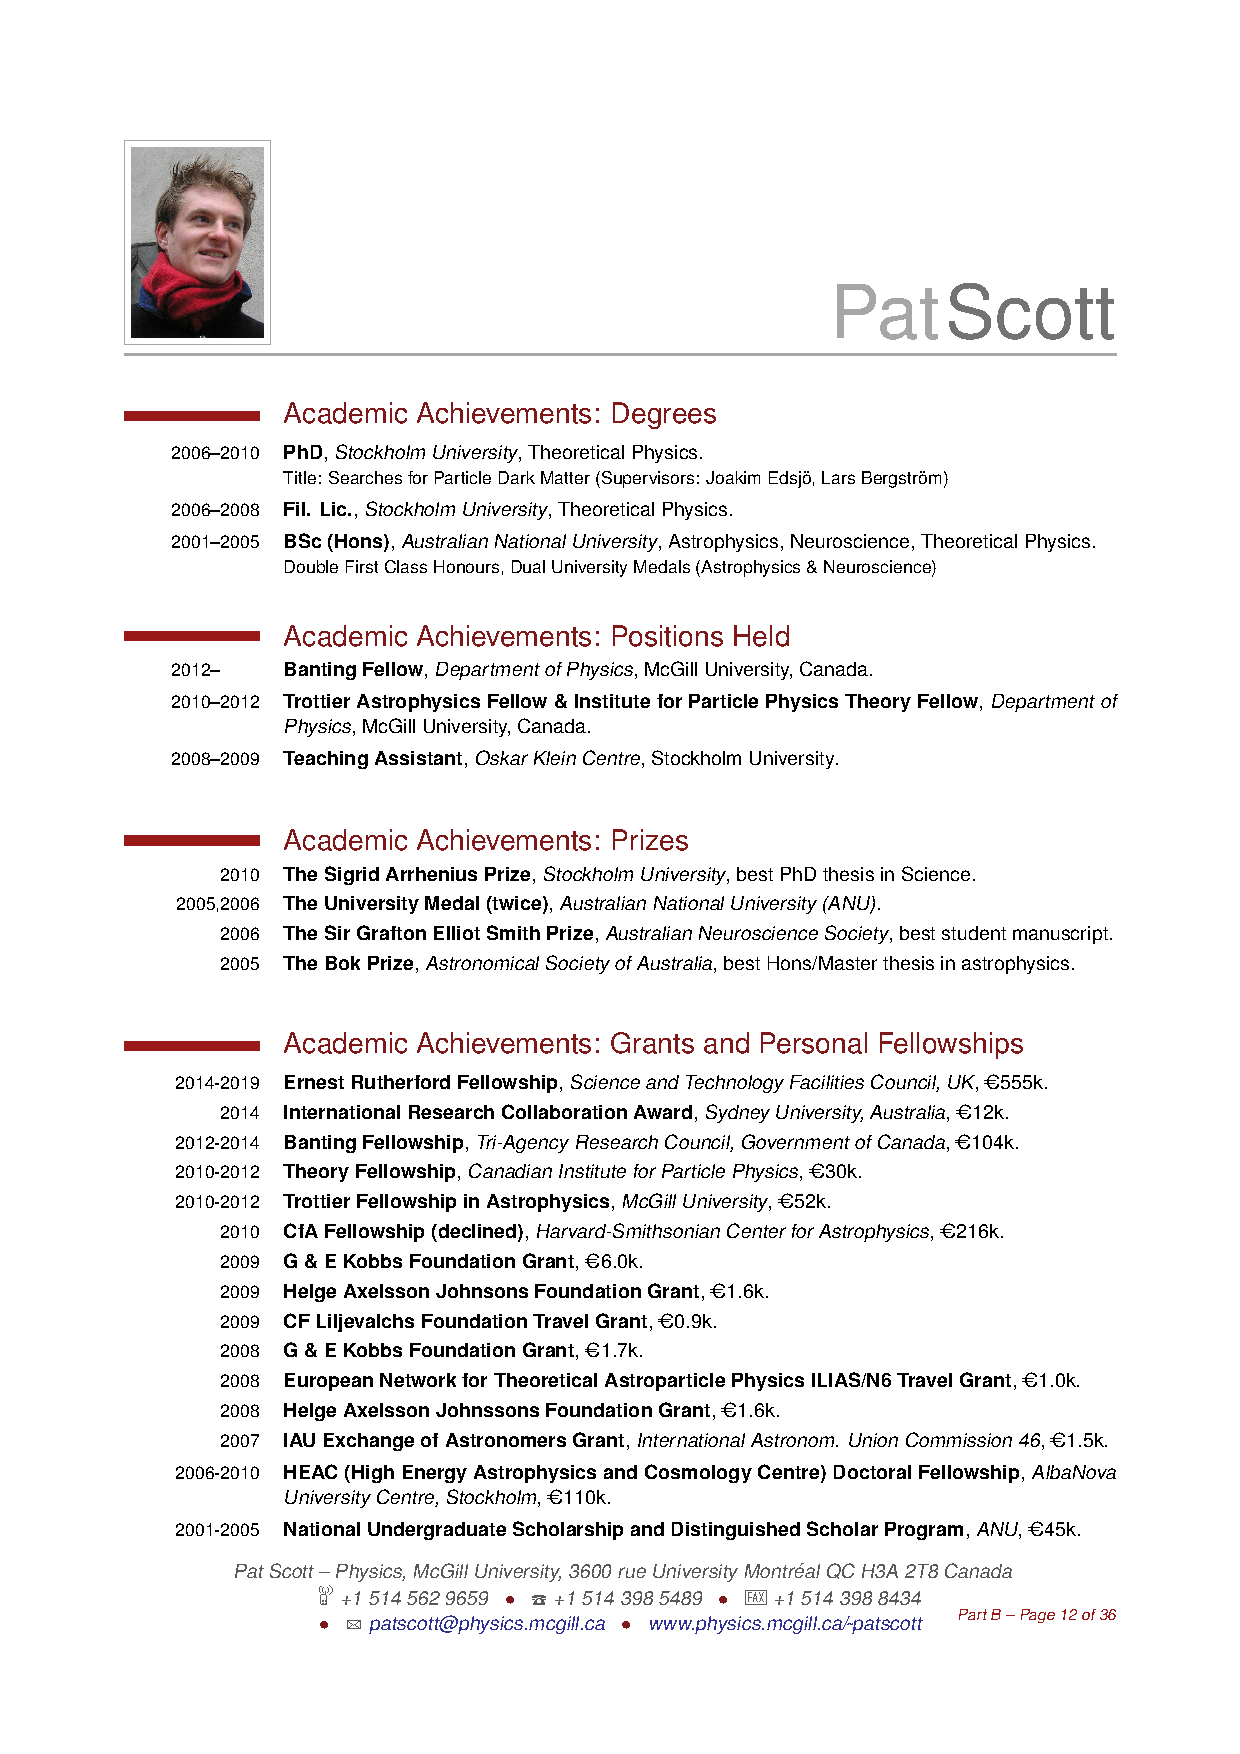
\includepdf[pages=-]{CV}

%%%%%%%%%%%%%%%%%%%%%%%%%%%%%%%%%%%%%%%%%%%%%%%%%%%%%%%%%%%%%%%%%%%%%%%%%%%%%%%%%%%%%%%%
%%%%%%%%%%%%%%%%%%%%%%%%%%%%%%%%%%%%%%%%%%%%%%%%%%%%%%%%%%%%%%%%%%%%%%%%%%%%%%%%%%%%%%%%
\newpage
\section{Implementation}
\begin{xcomment}  
Maximum 4 pages
\end{xcomment}

%%%%%%%%%%%%%%%%%%%%%%%%%%%%%%%%%%%%%%%%%%%%%%%%%%%%%%%%%%%%%%%%%%%%%%%%%%%%%%%%%%%%%%%%
\subsection{Quality of host organisation, including adequacy of facilities}

\begin{xcomment}
The host institution must explain the level of experience on the
research topic proposed, including international collaborations of
relevance. Information provided should include participation in
projects, publications, patents and any other relevant
results. Information on the capacity to provide training in
complementary skills that can further aid the fellow in the
integration period and beyond should be included. The host needs to
specify what are the infrastructures available and whether these can
respond to the needs set by the execution of the project.
\end{xcomment}

Imperial College London offers the perfect combination of professional and scientific environments, computational resources and location.

\textbf{An ideal professional environment.} I will partake in decision-making and student supervision in the Astrophysics Group at Imperial as if already a permanent member of staff.  My career path will be factored into the Group's long-term strategy, with the intention of retaining me as a lecturer.  I will have opportunities to lecture graduate and undergraduate courses, and to officially co-supervise graduate students.  I will be supported with extensive feedback from experienced faculty on applications for research funding, and on the process of building my own independent research group.  I will have access to staff development workshops providing training in complementary skills like project management, leadership, communication and grant writing.

\textbf{Vast expertise relevant to my research.} 
I will collaborate closely and co-supervise students with Roberto Trotta, who has extensive experience in dark matter and global fits \cite{Trotta08, SuperbayesXENON100, BertoneLHCDD, Strege12, Strege13}. My research program will both enhance the activities of and benefit greatly from the new Imperial Centre for Inference and Cosmology, as I work with Alan Heavens, David van Dyk, et al in improving the numerical and statistical optimisation methods central to my global fits.  With Henrique Araujo and Tim Sumner, leading figures in the ZEPLIN/LUX direct detection project \cite{ZEPLINIII}, I will ensure that results of LUX and other direct detection experiments are correctly included in my global fits, in the most detailed way possible: at the level of single nuclear recoil events. I will draw on the Imperial CMS group in developing collider likelihood modules, particularly when optimising fast detector simulations and applying comparable analysis event cuts to the proprietary CMS analyses.  Roberto Trotta, Andrew Jaffe, Jonathan Pritchard, Daniel Mortlock, Carlo Contaldi and Arttu Rajantie will provide excellent cosmological expertise, including strong involvement with the Planck Collaboration \cite{PlanckCosmology}.  Michael Duff and the Theory Group will be invaluable points of reference as quantum field theory questions arise when I and my new group implement many new particle models in the GAMBIT code.

\textbf{Priority access to over 10,000 cores of cluster computing power.}
Imperial's High Performance Computing (HPC) facilities consist of three main computing clusters, boasting over 10,000 total processor cores, a priority queue on a subset for the Astrophysics Group, and the ability to run single jobs on over 3,000 of the latest CPU cores.  This sort of computing infrastructure is essential for the highly computationally demanding, high-dimensional global fits that I will be carrying out in the course of this project.  Running code on the Imperial HPC infrastructure will provide a perfect development base and the experience necessary to apply for time on the UK Science and Technology Facilities Council HECToR supercomputing facility.

\textbf{A productive geographical location.}
The greater London area also boasts strong cosmology and particle phenomenology groups at University College London and King's College London respectively, leading to good prospects for future collaboration on scientific projects and organisation of conferences and workshops.

%%%%%%%%%%%%%%%%%%%%%%%%%%%%%%%%%%%%%%%%%%%%%%%%%%%%%%%%%%%%%%%%%%%%%%%%%%%%%%%%%%%%%%%%
\subsection{Feasibility and credibility of the project, including work plan}

\begin{xcomment}
Provide a work plan that includes the goals that can help assess the
progress of the project taking into account also non-research related
activities that will be part of the integration project in the frame
of the employment (e.g. teaching, etc). Mention the arrangements made
in terms of supporting the integration phase of the fellow providing a
career development plan where applicable. Where appropriate, describe
the approach to be taken regarding the intellectual property that may
arise from the research project.

In addition, the host institution is requested to provide an
indicative budget covering the duration of the project and related to
its implementation and to the planned research activities. This
indicative breakdown of costs should refer to the overall total costs
of the project, regardless of the source of funding, including the
expected EU contribution and the host's own budget, with no
distinction (preferably using a table):

\begin{itemize}
\item Salary of the researcher
\item Other salary costs (e.g. assistants, technicians) 
\item Travel costs
\item Consumables
\item Management activities 
\item Overheads
\item Others (to be listed where applicable)  
\end{itemize}

As the project must be described in full regardless of the source of
funding, the relevance of the EU financial contribution for the
implementation of the project itself should be clearly highlighted.
\end{xcomment}

\subsubsection{Work Plan}

The following work plan lists the goals and milestones of my core global-fit research program over the four years of the CIG, and the further fifth year funded by my UK Science and Technology Facilities Council (STFC) Ernest Rutherford Fellowship.  Concrete deliverables are \textcolor{red}{listed in red}.

\noindent\textbf{Years 1--2} Develop:\\
$\phantom{xx}\bullet$ core second-generation global fitting code\\
$\phantom{xx}\bullet$ likelihood modules: first LHC (few channels), direct detection, indirect detection\\
$\phantom{xx}\bullet$ differential evolution scanner\\
\textcolor{red}{Publish:}\\
$\phantom{xx}\bullet$ \textcolor{red}{indirect detection likelihood code package paper}\\
$\phantom{xx}\bullet$ \textcolor{red}{direct detection likelihood code package paper}\\
$\phantom{xx}\bullet$ \textcolor{red}{differential evolution code paper}\\
\noindent\textbf{Year 3}\\ 
$\phantom{xx}\bullet$ \textcolor{red}{Publish phenomenological MSSM analyses}\\
$\phantom{xx}\bullet$ \textcolor{red}{first public release of code}\\
\noindent\textbf{Year 4} Add/update observables:\\
$\phantom{xx}\bullet$ all LHC channels\\
$\phantom{xx}\bullet$ cosmic rays + propagation models\\
$\phantom{xx}\bullet$ gamma-rays\\
$\phantom{xx}\bullet$ neutrino telescope\\
$\phantom{xx}\bullet$ CMB limits on DM annihilation\\
Add theories:\\
$\phantom{xx}\bullet$ supersymmetry-breaking mediation models\\
$\phantom{xx}\bullet$ extra dimensions\\
$\phantom{xx}\bullet$ Two Higgs Doublet Models\\
$\phantom{xx}\bullet$ effective DM models\\
\noindent\textbf{In the year following completion of the CIG (funded by STFC)}\\
\textcolor{red}{Complete and publish (for all theories):}\\ 
$\phantom{xx}\bullet$ \textcolor{red}{global parameter analyses}\\
$\phantom{xx}\bullet$ \textcolor{red}{extensive model comparison}

\vspace{3mm}
\noindent My goal is to officially supervise at least one student and a postdoc on this project during this period, but that is contingent upon funding for their salaries (which I have applied for from STFC).  It is also worth noting that the GAMBIT Collaboration already contains a number of students and postdocs, whom I have already naturally come to mentor.  I will therefore be engaged in significant supervision, as an integrated component of my research program, regardless of whether I obtain money for a postdoc and/or student of my own (and therefore stand to gain that experience anyway, albeit not at the same level as if I were to supervise them officially).

Although my STFC fellowship formally frees me from teaching obligations for a period of 5 years, I intend to teach a small amount (not more than one course per year), in order to increase my teaching experience, better recruit students, and thereby enhance my integration into the Department of Physics on a permanent basis.  Including outreach and supervisory activities as integrated parts of this project, during the timeframe of my CIG I expect to spend 90\% of my time on the research program outlined here.

\subsubsection{Career Development Plan}

My STFC Ernest Rutherford Fellowship carries with it an expectation that at the completion of the Fellowship, Imperial College will do everything in its power to employ me as a lecturer -- although this is not guaranteed.  My performance will be reviewed annually by my line manager (R.\ Trotta) using Imperial's Personal Review and Development Plan process.\footnote{\href{http://www3.imperial.ac.uk/hr/workingatimperial/career/promotion/prdp}{http://www3.imperial.ac.uk/hr/workingatimperial/career/promotion/prdp}}  Subject to good performance, the Astrophysics Group will include my promotion to lecturer as part of their Annual Strategy Document, which outlines the Group's vision for the next 5 years, and strongly influences the Department's planning for the future.

I will be trained in the additional non-research skills required in a permanent academic career, to maximise my argument for a permanent position during the course of the fellowship.  I will be given managerial experience by being integrated into the faculty structure of the Astrophysics Group and their planning and decision-making processes, and by supervising/co-supervising Masters and PhD students.  I will have access to a wide range of formal staff development workshops covering project management, leadership, communication and grant writing.\footnote{\href{http://www3.imperial.ac.uk/staffdevelopment}{http://www3.imperial.ac.uk/staffdevelopment}}  I will gain additional experience in grant writing, and improve these skills with detailed feedback from senior faculty.  I will increase my teaching experience, both at undergraduate and graduate level.

\subsubsection{Indicative budget}

`STFC' in the table below refers to the contribution of my STFC Ernest Rutherford Fellowship.

\vspace{3mm}
\begin{tabular}{|l|r|r|r|}\hline
Budget Item					& STFC ({\sf \euro})	& CIG ({\sf \euro}) 	& Total ({\sf \euro})\\\hline
Researcher salary				& 219\,086	& 37\,524	& 273\,857	\\
Travel costs					& 7\,619	& 38\,476	& 48\,000	\\
Visitor costs					& --		& 16\,000	& 16\,000	\\
Organisation of GAMBIT Collaboration Meeting	& --		& 6\,000	& 6\,000	\\
Outreach					& --		& 2\,000	& 2\,000	\\
Overheads and estate costs			& 207\,848	& --		& 259\,810	\\
Infrastructure technicians			& 4\,556	& --		& 5\,695	\\
Relocation					& 2\,857	& --		& 3\,572	\\
Computing hardware				& 4\,762	& --		& 5\,953	\\\hline
\textbf{Totals}					& 446\,728	& 100\,000	& 620\,887	\\\hline
\end{tabular}

\vspace{3mm}
\noindent \textbf{Salary:} Includes superannuation (pension contributions).\\
\textbf{Travel costs:} GAMBIT Collaboration meetings occur every 9 months in Europe, Australia or North America, and last a full week.  Attending from the UK will cost approximately \euro4000 per year.  The remaining \euro8000 I have budgeted per year covers attendance at one intercontinental conference (\euro2000), two European conferences (\euro1250 each), a 2-week visit to another GAMBIT institute (\euro2000), and miscellaneous domestic travel/conferences (\euro1500).\\
\textbf{Visitor costs:} This covers a 2-week visit per year by another GAMBIT member (\euro2500) and a week-long visit by another one or two European researchers, with whom interacting will enhance my research program (\euro1500).  The latter might be e.g. a theorist responsible for inventing a particular model I am implementing in GAMBIT, or an experimentalist familiar with a given dataset I am attempting to integrate into my fits.\\
\textbf{Organisation of GAMBIT Collaboration Meeting} I will use this money to host a GAMBIT Collaboration Meeting in the UK.  This will boost both my integration into the UK particle/astrophysics community, and my leadership within GAMBIT.\\
\textbf{Outreach:} Materials and advertising costs associated with the activities outlined in Sec.\ \ref{outreach}.\\
\textbf{Overheads:} The Imperial College Department of Physics does not deduct overheads from CIGs.
\textbf{Technicians:} Broad-spectrum IT support services provided by Imperial ICT.\footnote{\href{http://www3.imperial.ac.uk/ict}{http://www3.imperial.ac.uk/ict}}\\
\textbf{Relocation:} Airfares and removal costs from Montreal.\\
\textbf{Computing hardware:} Two high-end laptops (one each at the start of years one and three) and associated ergonomic peripherals, required for developing GAMBIT code.

\vspace{3mm}
\noindent \textbf{Impacts of CIG funds:} CIG funds will allow Imperial College to employ me at approximately the salary level of a starting lecturer. Having external funding for this salary level will make me a much more attractive prospect for future integration into a permanent academic research career at the College.  Availability of CIG funds will make me able to travel to collaborate with other GAMBIT members at their home institutes (typically within Europe), to GAMBIT Collaboration Meetings, and to a broad range of conferences and meetings where I will be able to present my results.  Travel is essential for my reintegration into the European Research Area, as it will allow me to a) lead GAMBIT by attending the Collaboration Meetings, b) make significant progress on my project together with GAMBIT collaborators at their home institutes, and c) increase familiarity of my work within the European community.  The CIG funds will also provide a visitor's budget for me at Imperial, allowing me to invite GAMBIT members to work with me there, as well as other relevant experts from outside the Collaboration.  The CIG will allow me to organise one GAMBIT Collaboration Meeting in the UK as well.  Without the CIG, I would not be able to attend GAMBIT Collaboration Meetings without financial assistance from the organisers, nor would it be possible to host a GAMBIT meeting myself. If this situation persisted for much longer than a year or two, my position as leader of the Collaboration would likely become untenable, gravely damaging my prospects for effective reintegration into the EU.  I would also have no outreach budget without a CIG.

\subsubsection{Intellectual property: The GAMBIT Data Management Plan}

Data products are the underlying global-fit code (consisting of modules: Core, Dark Matter, etc), reduced experimental data used as input to physics modules, and sets of samples from scans of BSM theories.  GAMBIT codes, documentation and datafiles will be publicly available on Hepforge (the standard for HEP software) with a \texttt{git} interface administered via GitHub, and will remain available for the lifetime of Hepforge.  Individual physics modules will be available, configured for standalone use.  Samples from parameter spaces produced for GAMBIT papers will be posted on the GAMBIT Collaboration website (served from Hepforge) as papers appear on the arXiv.  All materials will be stored in triplicate on Hepforge, GitHub and a local server.

%%%%%%%%%%%%%%%%%%%%%%%%%%%%%%%%%%%%%%%%%%%%%%%%%%%%%%%%%%%%%%%%%%%%%%%%%%%%%%%%%%%%%%%%
\subsection{Management: Practical arrangements for the implementation and management of the research project}

\begin{xcomment}
The applicant and the host institution should provide information on
how the implementation and management of the grant will be
achieved. The experts will be examining the practical arrangements
that can have an impact on the feasibility and credibility of the
project. A contingency plan, e.g. alternative activities, risk
management plan, should be mentioned.
\end{xcomment}

I will take care of day-to-day implementation and management of the project, as I develop the GAMBIT code, carry out physics analyses with it, and meet both in person and remotely with other members of the GAMBIT Collaboration to discuss strategies and progress.  Depending on my success in obtaining additional funding, this will also hopefully include regular weekly group meetings with postdocs and/or students.  I will report on progress to the rest of the GAMBIT Collaboration -- and monitor others' progress -- on a regular basis via our monthly all-Collaboration Vidyo meetings, our 9-monthly face-to-face Collaboration Meetings, and our monthly/fortnightly Vidyo meetings in the different constituent Working Groups (Core/Models, Collider, Dark Matter and Scanner; I lead the Core/Models WG and am a member of the other three).  Extensive policies and procedures for conflict resolution, publication, presentations, membership changes and coding conventions have all been agreed on and laid down in detail in the GAMBIT Collaboration Policies Document.

I will report progress to other faculty in the Astrophysics Group at longer intervals, but not less than every six months.  I will operate as a member of the Astrophysics Group, but will make special effort to also engage strongly with the High Energy Group and the Theory Group, attend their seminars and encouraging them to attend Astrophysics events, and make sure that research at the boundaries of the interests of the three groups is well-represented in each of their speaker rosters.  I will have the assistance of two Group Secretaries, a Departmental Research Operations Manager, and a suite of computing infrastructure technicians provided by Imperial ICT services.

\textbf{Risks and Contingencies:} The beauty of a global-fit approach to phenomenology is that the overall success of the research program is quite robust with respect to most `standard' risks.  Catastrophic failure of an experiment is not likely to derail or even significantly delay the program, as it draws on many different experiments.  Failure to discover dark matter or new physics in the next few years, whilst disappointing, will not prevent me from combining all searches into holistic analyses that determine and then compare the overall status of different models and their agreement or disagreement with data.  The most significant risk is that some non-faculty members of GAMBIT might not obtain ongoing employment, and choose to leave physics during the course of this grant.  As much as I hope this does not happen, I have identified strong prospective replacements for all members for whom I consider this a significant risk.


%%%%%%%%%%%%%%%%%%%%%%%%%%%%%%%%%%%%%%%%%%%%%%%%%%%%%%%%%%%%%%%%%%%%%%%%%%%%%%%%%%%%%%%%
%%%%%%%%%%%%%%%%%%%%%%%%%%%%%%%%%%%%%%%%%%%%%%%%%%%%%%%%%%%%%%%%%%%%%%%%%%%%%%%%%%%%%%%%
\newpage
\section{Impact}
\begin{xcomment}  
Maximum 5 pages
\end{xcomment}

%%%%%%%%%%%%%%%%%%%%%%%%%%%%%%%%%%%%%%%%%%%%%%%%%%%%%%%%%%%%%%%%%%%%%%%%%%%%%%%%%%%%%%%%
\subsection{Contribution to research excellence by attracting and retaining first class researchers}
\begin{xcomment}
Describe how the researcher's integration will contribute to enhancing
EU scientific excellence.
\end{xcomment}

My research program will take a fledgling field of research, namely BSM global fits, and transform it into a standard phenomenological tool used by theorists and experimentalists throughout particle and astroparticle physics.  The GAMBIT Collaboration will be at the forefront of this movement, providing the scientific leadership and computational tools required to ``bring global fitting to the masses''.  With the majority of GAMBIT members already located in Europe, my move to the UK with a CIG will mean that Europe will be the epicentre of this transformation.  GAMBIT will ensure that Europe leads the world in understanding the overall combined implications of experimental searches for BSM physics.  This will secure the global lead that Europe already holds in collider searches for new physics through the activities of CERN, and in astroparticle searches for particle dark matter, due to strong investment in astroparticle physics through bodies such as ApPEC/ASPERA.

By centring GAMBIT on Europe, we will attract first class talent to the European Research Area from other third countries, to work as doctoral, postdoctoral and senior researchers on GAMBIT.  One such researcher, presently an extremely strong finishing doctoral student in Australia and GAMBIT member, will almost certainly also join Imperial College if I am successful in obtaining funding for a postdoctoral researcher.  This is a story repeated throughout the Collaboration, all around Europe: in Oslo, Stockholm, Geneva, Zurich, Amsterdam and Glasgow.  My relocating to Europe will strengthen the GAMBIT Collaboration as a whole by co-locating its leader and the bulk of its membership.  This will greatly increasing GAMBIT's likelihood of success, and therefore the prospects of GAMBIT institutes throughout Europe being able to attract and retain first class researchers.

%%%%%%%%%%%%%%%%%%%%%%%%%%%%%%%%%%%%%%%%%%%%%%%%%%%%%%%%%%%%%%%%%%%%%%%%%%%%%%%%%%%%%%%%
\subsection{Potential and quality of the researcher's long term professional integration in Europe}
\begin{xcomment}
Describe the prospects for a lasting professional integration for the
researcher, namely the type of work agreement to be provided, the
length and the full time dedication:

\begin{itemize}
\item expected impact on the future career development of the researcher;
\item expected length of the employment contract;
\item attractiveness of the remuneration package.
\end{itemize}

Please describe the potential for developing lasting integration of
the researcher following the end of the project.
\end{xcomment}

The contract offered to me by Imperial is for 5 years of full-time research, with a strong likelihood of conversion to a continuing appointment towards the end of that contract.  I will be hired at level C, spine point 38.  Employees at Imperial rise one spine point per year.  Starting lecturers begin at level C, spine point 39.  I will therefore be hired at a remuneration level just one year behind a permanent lecturer, and will in fact progress to spine point 39 only 7 months after starting my contract.  This is not only an attractive pay scale (corresponding to \euro51\,260 per year after pension deductions and before tax), but bodes very well for my future prospects of obtaining permanent employment at Imperial.

I will receive specific professional training to aid me in attaining lasting integration following the termination of my CIG: managerial experience through a seat at the decision-making table of the Astrophysics Group (together with the group's faculty members), teaching experience by lecturing classes and running tutorials for undergraduate and graduate students, supervisory experience though GAMBIT and hopefully, also my own PhD and Masters students, and grant-writing coaching from senior members of the Astrophysics Group.

By facilitating my continued leadership of the GAMBIT Collaboration, through the software development phase and on to the production and dissemination of ground-breaking scientific results, this CIG will place me in an enviable position in terms of long-term professional integration in Europe.  At the end of the integration period, I will be positioned to apply GAMBIT to an even broader range of models and physical problems than I have described here, and incorporate yet wider and wider areas of physics as potential constraints (e.g. neutrino-sector, cosmological and stellar constraints).  I will be recognised as one of the leading contributors to many of the most important reference papers in BSM physics of the next decades, and the lead author of a computer code that should become one of the most important tools in particle or astroparticle phenomenology.  Through GAMBIT, this profile and the conference presentations I will give in the course of the CIG, I will be able to develop a strong and diverse network of collaborators throughout Europe.  Together, these aspects will ensure my successful professional integration into the European Research Area.

%%%%%%%%%%%%%%%%%%%%%%%%%%%%%%%%%%%%%%%%%%%%%%%%%%%%%%%%%%%%%%%%%%%%%%%%%%%%%%%%%%%%%%%%
\subsection{Potential of transferring knowledge to the host organisation}
\begin{xcomment}
Outline the capacity for transferring the knowledge previously
acquired to the host.
\end{xcomment}

There are three specific topics where my technical expertise is highly complementary to that already present at Imperial:
\begin{itemize}
\item theories for new physics and particle dark matter,
\item indirect experimental searches for particle dark matter,
\item numerical methods in physics.
\end{itemize}
The first two of these I will transfer effectively by collaborating with other academics in the Astrophysics, High Energy and Theory Groups, in particular on global fits with Roberto Trotta and the LUX/ZEPLIN direct detection subgroup.  Numerical methods are an area of strength at Imperial, in part due to the expertise contained in the Imperial Centre for Inference and Cosmology (ICIC) -- but there are certain specialised methods, such as genetic algorithms and differential evolution, where I stand to contribute new expertise to Imperial's existing knowledge base.  Topics such as this I will transfer knowledge of by way of an informal ICIC seminar or discussion session.  I have also thought in rather a lot of depth about a number of more `standard' numerical methods used for everyday research tasks like interpolation, integration and root-finding, in preparing my Numerical Methods in Physics course at McGill.  I am therefore better-placed than most to communicate and teach everyday research use of numerical methods to graduate students.  My intention is therefore to transfer this knowledge by offering graduate students in the Department of Physics a modified version of my Numerical Methods course at least once during the course of my CIG.

Finally, I am unusually well-connected in the particle dark matter community for a person at my career stage, and in a slightly lesser way, also across astrophysics, high energy physics and astroparticle experiment more generally.  This is a form of knowledge that I have also been very successful at transferring to the institutes I work at, as evidenced by e.g. continued high attendance at the McGill Astroparticle Seminar Series (which I created).  Transferring this sort of `network knowledge' is important for the future career and collaboratory prospects of the students and postdocs in a Department, and for the general scientific benefit of all research staff.  My plan for transferring this knowledge to Imperial is to actively invite my contacts and collaborators to visit, give seminars and interact with members of the Department of Physics.


%%%%%%%%%%%%%%%%%%%%%%%%%%%%%%%%%%%%%%%%%%%%%%%%%%%%%%%%%%%%%%%%%%%%%%%%%%%%%%%%%%%%%%%%
\subsection{Capacity to develop lasting co-operation and collaboration with other countries}

\begin{xcomment}
Describe the potential for developing lasting cooperation with other
countries' research organizations.
\end{xcomment}

Within the context of the research program funded by my CIG, the GAMBIT Collaboration offers an obvious means by which to further develop lasting collaborative relationships with individual researchers and research communities in other countries.  Within the European Community, I will deepen my collaborative links with GAMBIT members in France, Germany, the Netherlands, Norway, Sweden, Switzerland and the UK, through return collaborative visits to each others' institutes to work on GAMBIT, as well as exchange and joint supervision of students to the same ends.  Beyond the EC, I will do the same with GAMBIT members in Australia and the US.  I have particularly strong links to the high energy (both theory and experiment)  and astrophysics communities in Australia and the astroparticle community in Sweden, so will explore possibilities for future joint grant applications, training networks and research consortia with my contacts in both places during the course of the CIG.  

I will also retain strong links to McGill University and Canada, in theoretical cosmology and particle phenomenology.  I am in the process of preparing a joint research proposal to the FQRNT (the Quebec national research council) with members of the McGill faculty, on constraining theories that can produce both dark matter and cosmic strings, using observational cosmology and searches for particle dark matter.  If the proposal is accepted, I will be an external node of the research consortium based at Imperial, with the understanding that some of the grant monies will be used to exchange students and other personnel between McGill and Imperial.  That proposal links nicely with the research program I describe here, as both sets of constraints and the relevant models will be implementable naturally within the GAMBIT framework with a minimum of modification, allowing our proposed analyses to be performed very straightforwardly.

These activities would benefit students and academic staff at Imperial by bringing high class scientific visitors to speak, interact and potentially form new collaborations of their own with Imperial College research staff.  More concretely though, my own contacts in GAMBIT will be of great benefit to some members of the Department at Imperial, because I envisage them actually joining the GAMBIT Collaboration themselves.  This of course goes for any students or postdocs I hire myself to work on this project, but potentially also for additional interested faculty and/or postdocs already at Imperial.  This would make Imperial an even more active and intense node of GAMBIT activity, and would open up the same suite of international collaborators that I already benefit from to my colleagues at Imperial as well.

%%%%%%%%%%%%%%%%%%%%%%%%%%%%%%%%%%%%%%%%%%%%%%%%%%%%%%%%%%%%%%%%%%%%%%%%%%%%%%%%%%%%%%%%
\subsection{Plans for dissemination and exploitation of results}

\begin{xcomment}
This section should include a list of planned dissemination
activities, such as publications, conferences, workshops, and
websites.
\end{xcomment}

I will disseminate my research primarily by publishing it in top-tier journals like JCAP and JHEP, and presenting it at international conferences like ICHEP, Moriond, IDM and TeVPA.  GAMBIT papers, results, datasets and code will all be made available from Hepforge and the GAMBIT website \href{http://gambit.hepforge.org}{gambit.hepforge.org}.  Other researchers will be able to further exploit GAMBIT results by reprocessing them with the public GAMBIT code, to e.g. add additional observables or datasets.  The code itself will follow specific design principles of flexibility and easy extensibility, so as to encourage users to develop their own likelihood, observable, scanner or theory modules, and then contribute them back to the main GAMBIT codebase for the entire community to use.  

One additional means by which the results of global fits can be exploited is to perform fits of \textit{proposed} experiments, and compare different experimental designs in terms of their ability to constrain/detect different particle theories.  I intend to do this anyway for its scientific value, but I also mean to submit the results of similar exercises to particle/astroparticle funding bodies and planning committees.  These will include STFC in the UK and ASPERA/ApPEC at the EU level. This information is highly valuable to such bodies, as it can be used to make informed choices between different proposed experiments and experimental configurations.


%%%%%%%%%%%%%%%%%%%%%%%%%%%%%%%%%%%%%%%%%%%%%%%%%%%%%%%%%%%%%%%%%%%%%%%%%%%%%%%%%%%%%%%%
\subsection{Impact of the proposed outreach activities}
\label{outreach}

\begin{xcomment}
In order to promote communication between the scientific community and
the general public and increase awareness of science, various outreach
activities should be outlined in this section. For the planned
outreach activities, their expected impact should be explained in the
proposal. For examples, see box on outreach activities below.
\end{xcomment}

The Imperial Astrophysics Group has a strong history of innovative outreach activities. I will contribute to these both as an organiser and public presenter, with special focus on three activities.

\subsubsection{Interactive GAMBIT Multimedia Application}
 
\textbf{Outreach Activities Plan:} I plan to develop an interactive, computer-based exposition of the roles and impacts of different experiments around the world in the hunt for new physics, based on the results of my global fits.  This will be arranged as a research project for a group of first or second-year undergraduates.  It might appear in a science museum, on an Imperial webpage, or taken on tour to e.g. schools in disadvantaged areas.\vspace{3mm}

\noindent\textbf{Expected Impacts:}  Schoolchildren who use the interactive application will learn about some of the exciting particle/astroparticle experiments going on around the world, and the progress made so far in the search for new physics.  By highlighting the complementarity of the different experiments, the application will help them learn to see science as a global, international and co-operative endeavour.  By featuring large experiments in exotic locations (e.g. HESS in Namibia, IceCube in Antarctica, Auger at the foot of the Andes), they will also learn a little of parts of the world that they are unlikely to be familiar with already.  More generally, the application should be fun, and therefore promote enthusiasm for physics.

\subsubsection{Workshop Day}
 
\textbf{Outreach Activities Plan:} I will hold a Workshop Day for undergraduate university students, in order to introduce them to astroparticle and particle phenomenology, and the opportunities for combining astrophysics and particle physics in the future if they choose to pursue research careers.\vspace{3mm}

\noindent\textbf{Expected Impacts:} Students will learn of the current state of real physics research in astroparticle and particle physics, gain insight into what it is like to carry out research, and become aware of the opportunities for combining astronomy and particle physics in their future careers.

\subsubsection{Website/e-Newsletter}

\textbf{Outreach Activities Plan:} When the GAMBIT software is released for public download, I will author a Wikipedia entry on the GAMBIT Collaboration and the code.\vspace{3mm}

\noindent\textbf{Expected Impacts:} By reading the Wikipedia page, the general public will be able to find out some general information about GAMBIT, some of its more impressive technical/computational aspects, and its contributions to the discovery/exclusion of popular particle theories.


%%%%%%%%%%%%%%%%%%%%%%%%%%%%%%%%%%%%%%%%%%%%%%%%%%%%%%%%%%%%%%%%%%%%%%%%%%%%%%%%%%%%%%%%
%%%%%%%%%%%%%%%%%%%%%%%%%%%%%%%%%%%%%%%%%%%%%%%%%%%%%%%%%%%%%%%%%%%%%%%%%%%%%%%%%%%%%%%%
\newpage
\section{Ethical Issues}
\begin{xcomment}
  No page limit.

  NOTE: the original template by the EU contains more information regarding ethics.
\end{xcomment}

ETHICAL ISSUES TABLES
\vspace{5mm}

\begin{tabular}{|p{10cm}|p{1cm}|p{1cm}|}\hline
\bf Research on Human Embryo/ Foetus									& YES	& Page	\\\hline
Does the proposed research involve human Embryos?							&	&	\\\hline
Does the proposed research involve human Foetal Tissues/ Cells?						&	&	\\\hline
Does the proposed research involve human Embryonic Stem Cells (hESCs)?					&	&	\\\hline
Does the proposed research on human Embryonic Stem Cells involve cells in culture?			&	&	\\\hline
Does the proposed research on Human Embryonic Stem Cells involve the derivation of cells from Embryos?	&	&	\\\hline
I CONFIRM THAT NONE OF THE ABOVE ISSUES APPLY TO MY PROPOSAL						&X	&N/A	\\\hline
\end{tabular}
\vspace{3mm}

\begin{tabular}{|p{10cm}|p{1cm}|p{1cm}|}\hline
\bf Research on Humans											& YES	& Page	\\\hline
Does the proposed research involve children?								&	&	\\\hline
Does the proposed research involve patients?								&	&	\\\hline
Does the proposed research involve persons not able to give consent?					&	&	\\\hline
Does the proposed research involve adult healthy volunteers?						&	&	\\\hline
Does the proposed research involve Human genetic material?						&	&	\\\hline
Does the proposed research involve Human biological samples?						&	&	\\\hline
Does the proposed research involve Human data collection?						&	&	\\\hline
I CONFIRM THAT NONE OF THE ABOVE ISSUES APPLY TO MY PROPOSAL						&X	&N/A	\\\hline
\end{tabular}
\vspace{3mm}

\begin{tabular}{|p{10cm}|p{1cm}|p{1cm}|}\hline
\bf Privacy												& YES	& Page	\\\hline
Does the proposed research involve processing of genetic information or personal 
data (e.g. health, sexual lifestyle, ethnicity, political opinion, religious or 
philosophical conviction)?										&	&	\\\hline			
Does the proposed research involve tracking the location or observation of people?			&	&	\\\hline
I CONFIRM THAT NONE OF THE ABOVE ISSUES APPLY TO MY PROPOSAL 						&X	&N/A	\\\hline
\end{tabular}
\vspace{3mm}

\begin{tabular}{|p{10cm}|p{1cm}|p{1cm}|}\hline
\bf Research on Animals											& YES	& Page	\\\hline
Does the proposed research involve research on animals?							&	&	\\\hline
Are those animals transgenic small laboratory animals?							&	&	\\\hline
Are those animals transgenic farm animals?								&	&	\\\hline
Are those animals non-human primates?									&	&	\\\hline
Are those animals cloned farm animals?									&	&	\\\hline
I CONFIRM THAT NONE OF THE ABOVE ISSUES APPLY TO MY PROPOSAL						&X	&N/A	\\\hline
\end{tabular}
\vspace{3mm}

\begin{tabular}{|p{10cm}|p{1cm}|p{1cm}|}\hline
\bf Research Involving Developing Countries								& YES	& Page	\\\hline
Does the proposed research involve the use of local resources (genetic, animal, plant, etc)?		&	&	\\\hline
Is the proposed research of benefit to local communities (e.g. capacity building,
access to healthcare, education, etc)?									&	&	\\\hline
I CONFIRM THAT NONE OF THE ABOVE ISSUES APPLY TO MY PROPOSAL						&X	&N/A	\\\hline
\end{tabular}
\vspace{3mm}

\begin{tabular}{|p{10cm}|p{1cm}|p{1cm}|}\hline
\bf Dual Use												& YES	& Page	\\\hline
Research having direct military use									&	&	\\\hline
Research having the potential for terrorist abuse							&	&	\\\hline
I CONFIRM THAT NONE OF THE ABOVE ISSUES APPLY TO MY PROPOSAL						&X	&N/A	\\\hline
\end{tabular}
\vspace{3mm}

\begin{tabular}{|p{10cm}|p{1cm}|p{1cm}|}\hline
\bf Consistency with part A										& YES	& NO	\\\hline
I CONFIRM THAT THE INFORMATION GIVEN IN THIS TABLE IS
CONSISTENT WITH THE INFORMATION PROVIDED ON ETHICS IN PART A, PAGE A1					&X	&N/A	\\\hline
\end{tabular}
\vspace{3mm}

\section{Bibliography}
\bibliography{DMbiblio,SUSYbiblio,AbuGen,CosmoSF}

%%%%%%%%%%%%%%%%%%%%%%%%%%%%%%%%%%%%%%%%%%%%%%%%%%%%%%%%%%%%%%%%%%%%%%%%%%%%%%%%%%%%%%%%
%%%%%%%%%%%%%%%%%%%%%%%%%%%%%%%%%%%%%%%%%%%%%%%%%%%%%%%%%%%%%%%%%%%%%%%%%%%%%%%%%%%%%%%%
\cover{ENDPAGE}

\end{document}
